\documentclass{article}
\usepackage[utf8]{inputenc}
\usepackage[super,square]{natbib}
\usepackage{tabularx}
\usepackage{parskip}
\usepackage[margin=1.4in]{geometry}
\usepackage{csquotes}
\usepackage{amsmath}
\usepackage{amsfonts}
\usepackage{amsthm}
\usepackage{graphicx}
\usepackage{float}
\usepackage{hyperref}

\newcommand{\comment}[1]{}

\title{\vspace{-3cm} Statistical Learning Notes (ISLR)}
\author{}
\date{}

\comment{
- https://www.dataschool.io/15-hours-of-expert-machine-learning-videos/
- https://github.com/tdpetrou/Machine-Learning-Books-With-Python

Outline:
- Go over statistical learning book and add code snippets with python scikit learn
- Go over VC theory paper

2: Basics of stat learning and K Nearest Neighbor
3: Linear Regression
4: Logistic Regression and Linear Discriminant Analysis
5: Crossvalidation and bootstrapping
6: Regression improvements - stepwise regression, regularized regression and others
7: Non-linear methods - Polynomial regression, splines, general additive models
8: Decision Trees and Random Forests - bagging/boosting
9: Support Vector Machines
10: Unsupervised Learning- Principal components analysis and clustering
}

\begin{document}
\maketitle
\vspace{-1.5cm}

\tableofcontents
\newpage

\section{Introduction}
\subsection{A Brief History of Statistical Learning}
    \begin{enumerate}
        \item  At the beginning of the nineteenth century, Legendre and Gauss published papers on the method of least squares, which implemented the earliest form of what is now known as linear regression.
        \item In 1936 Fisher proposed linear discriminant analysis.
        \item In the 1940s, various authors put forth an alternative approach, logistic regression.
        \item In the 1950's, Frank Rosenblatt introduced the Perceptron and Neural Networks
        \item In the 1960's, various authors introduced Nearest Neighbor and K-means clustering.
        \item In the early 1970s, Nelder and Wedderburn coined the term generalized linear models for an entire class of statistical learning methods that include both linear and logistic regression as special cases.
        \item By the end of the 1970s, many more techniques for learning from data were available but all were almost all linear because of computational limitations.
        \item By the 1980s, computing technology had finally improved sufficiently that non-linear methods were no longer computationally prohibitive
        \item In mid 1980s Breiman, Friedman, Olshen and Stone introduced classification and regression trees,  including cross-validation for model selection.
        \item In 1986,  Hastie and Tibshirani introduced generalized additive models for a class of non-linear extensions to generalized linear models.
        \item In the 1990's Vapnik introduced Support Vector Machines.
        \item In the 2000's Brieman introduced Random Forest
        \item In the 2000's Hinton popularized Deep Learning and Artificial Neural Networks. 
    \end{enumerate}

\section{Statistical Learning}
\subsection{What is Statistical Learning}
$n$ -- number of observations or training data.

$p$ -- number of features or parameters.

$x_{ij}$ -- the value of the $j$th predictor, or input, for observation $i$

$X = (x_1, \dots, x_p)$  -- input vector a.k.a features, predictors, independent variables.

$\epsilon$  -- error term, independent of $X$ and has mean zero.

$Y = f(X) + \epsilon$ -- a model a.k.a. output or dependent variable.

$y_i$ -- the response variable for the $i$th observation

In essence, statistical learning refers to a set of approaches for estimating $f$. 

\subsubsection{Why Estimate \texorpdfstring{$f$}{f}?}
There are two main reasons for estimating $f$: prediction and inference. 

\subsubsection*{Prediction}

We can predict $Y$ using $\hat Y = \hat f(X)$ where $\hat f$ represents an estimate of $f$ and $\hat Y$ represents the resulting prediction for $Y$.

The accuracy of $\hat Y$ as a prediction for $Y$ depends on two quantities, the reducible error and the irreducible error. 

Reducible error is the result of an inaccurate statistical learning technique.

Irreducible error occurs because $Y$ is a function of $\epsilon$ which has variability that is dependent of $X$, so cannot be reduced via a statistical learning technique. Irreducible error may be larger than zero because of unmeasured variables or unmeasurable variation. The irreducible error will always provide an upper bound on the accuracy of our prediction for Y and is almost always unknown in practice.

\[
    E[(Y - \hat f (x))^2 | X = x] = \underbrace{[f(x) - \hat f(x)]^2}_{\text{Reducible}} + \underbrace{Var(\epsilon)}_{\text{Irreducible}} 
\]

Note, $E(Y - \hat Y)^2 = E[(Y - \hat f (x))^2 | X = x] = E[f(X) + \epsilon - \hat f(X)]^2$ represents the average, or expected value, of the squared difference between the predicted and actual value of $Y$ and $Var()$ represents the variance associated with the error term  $\epsilon$. We square the values in order to ignore the resulting sign when finding averages.


\subsubsection*{Inference}
Often, we are interested in understanding how $Y$ changes as a function of $X_1,\dots,X_p$. That is, when we vary the value of a given feature, what should the result look like. Now $\hat f$ cannot be treated as a black box, because we need to know its exact form.

Common questions occurring in this setting include,
\begin{itemize}
    \item Which predictors are associated with the response?
    \item What is the relationship between the response and each predictor?
    \item Can the relationship between Y and each predictor be adequately summarized using a linear equation, or is the relationship more complicated? 
\end{itemize}

Depending on whether our ultimate goal is prediction, inference, or a combination of the two, different methods for estimating $f$ may be appropriate though some modeling could be conducted both for prediction and inference.

Linear models allow for relatively simple and interpretable inference, but may not yield as accurate predictions as some other
approaches. In contrast, some highly non-linear approaches can potentially provide quite accurate predictions for $Y$ at the expense of a less interpretable model, for which inference is more challenging.

\subsubsection{How Do We Estimate \texorpdfstring{$f$}{f}?}

Our training data or observations can be represented as ${(x_1, y_1),(x_2, y_2),...,(x_n, y_n)}$ where $x_i = (x_{i_1}, x_{i_2},...,x_{i_p})^T$ are vectors and $y_i$ are typically scalars.

Then, we want to find a function $\hat f$ such that $Y \approx \hat f(X)$ for any observation $(X, Y)$

Broadly speaking, most statistical learning methods for this task can be characterized as either parametric or non-parametric

\subsubsection*{Parametric Methods}

This approach reduces the problem of estimating $f$ down to one of estimating a set of parameters.

\begin{enumerate}
    \item First, we make an assumption about the functional form, or shape, of $f$.
    
    \item After a model has been selected, we need a procedure that uses the training data to fit or train the model.
\end{enumerate}

For example, if we assume $f$ is linear, then $f(X) = \beta_0 + \beta_1X_1 + \beta_2X_2 + ... + \beta_p X_p$. To train the linear model, we need to estimate the parameters $\beta_0, \beta_1,..., \beta_p$, which is commonly done using (ordinary) least squares.


In general, fitting a more flexible model requires estimating a
greater number of parameters. These more complex models can lead to a phenomenon known as \textbf{overfitting} the data, which essentially means they follow the errors, or noise, too closely.

\subsubsection*{Non-parametric Methods}
Non-parametric methods do not make explicit assumptions about the functional form of $f$ and instead seek an estimate of $f$ that gets as close to the data points as possible while being reasonably smooth.

A very large number of observations (far more than is typically needed for a parametric approach) is required in order to obtain an accurate estimate for $f$. In order to fit a thin-plate spline, the data analyst must select a level of smoothness.

\subsubsection{The Trade-Off Between Prediction Accuracy and Model Interpretability}

\begin{figure}[H]
    \centering
    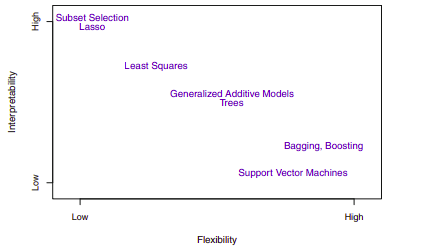
\includegraphics[width=11cm]{isl-figure-1.png}
\end{figure}


If we are mainly interested in inference, then restrictive models are much more interpretable.  In contrast, very flexible approaches, such as the splines and the boosting methods can lead to such complicated estimates of $f$ that it is difficult to understand how any individual predictor is associated with the response. 
Though there are clear advantages to using simple and relatively inflexible statistical learning methods when inference is the goal, the converse is not typically true. Instead we will often obtain more accurate predictions using a less flexible method. This phenomenon has to do with the potential for overfitting in highly flexible
methods.

\subsubsection{Supervised Versus Unsupervised Learning}
Most statistical learning problems fall into one of two categories: supervised or unsupervised.

In supervised learning, for each observation of the
predictor measurement(s) $x_i, i = 1,...,n$ there is an associated response measurement $y_i$. We wish to fit a model that relates the response to the predictors, with the aim of accurately predicting the response for future
observations (prediction) or better understanding the relationship between the response and the predictors (inference).

In contrast, unsupervised learning describes the situation in which for every observation $i = 1,...,n$, we observe a vector of measurements $x_i$ but no associated response $y_i$. It is not possible to fit a linear regression model, since there is no response variable to predict.  One statistical learning tool that we may use in this setting is cluster analysis which aims to ascertain, on the basis of $x_1,..., x_n$, whether the observations fall into relatively distinct groups.

In a semi-supervised learning problem, we wish to use a statistical learning method that can incorporate the $m$ observations for which response measurements are available as well as the $n - m$ observations for which they are not. 

\subsubsection{Regression Versus Classification Problems}
Variables can be characterized as either quantitative (taking on numerical values) or qualitative/categorical. We tend to refer to problems with a quantitative response as regression problems, while those involving a qualitative response are often referred to as classification problems, but it's not always clear-cut and many problems can use either responses. Whether the predictors are qualitative or quantitative is generally considered less important provided that any qualitative predictors are properly coded before the analysis is
performed.

\subsection{Assessing Model Accuracy}

\subsubsection{Measuring the Quality of Fit}
In order to evaluate the performance of a statistical learning method on a given data set, we need to quantify the extent to which the predicted response value for a given observation is close to the true response value for that observation.

The most commonly-used measure is the mean squared error (MSE), given by
\[
    MSE = \frac{1}{n} \sum_{i=1}^n (y_i - \hat f(x_i))^2.
\]

The MSE computed using the training data that was used to fit the model can be referred to as the training
MSE. We want to choose the method that gives
the lowest test MSE, i.e. we want $\hat f(x_0)$ to be approximately equal to $y_0$, where $(x_0, y_0)$ is a previously unseen test observation not used to train the statistical learning method.

As model flexibility increases, training MSE will decrease, but the test MSE may not. When a given method yields a small training MSE but a large test MSE, we are said to be overfitting the data. This is a fundamental property of statistical learning that holds regardless of the particular data set at hand and regardless of the statistical method being used. When we overfit
the training data, the test MSE will be very large because the supposed patterns that the method found in the training data simply don’t exist in the test data. 

One important method for estimating test MSE using the training data is cross-validation. 

\subsubsection{The Bias-Variance Trade-Off}

The expected test MSE, for a given value $x_0$, can always be decomposed into the sum of three fundamental quantities: the variance of $\hat f(x0)$, the squared bias of $\hat f(x_0)$ and the variance of the error variance bias terms. That is,

\[
    E \big (y_0 - \hat f(x_0) \big )^2 = Var( \hat f(x_0)) + [Bias( \hat f(x_0))]^2 + Var(\epsilon).
\]

$E \big (y_0 - \hat f(x_0) \big )^2$ defines the expected test MSE, computed by averaging the term over all possible values of $x_0$ in the test set.

In order to minimize the expected test error, we need to select a statistical learning method that simultaneously achieves low variance and low bias. 

Variance refers to the amount by which $\hat f$ would change if we estimated it using a different training data set. In general, more flexible statistical methods have higher variance. This is because changing any one of the data points may cause the estimate $\hat f$ to change considerably. A model with high variance does not generalize on the data which it hasn't seen before.

Bias refers to the error that is introduced by approximating a real-life problem, which may be extremely complicated, by a much simpler model. Generally, more flexible methods result in less bias

As a general rule, as we use more flexible methods, the variance will increase and the bias will decrease. The relative rate of change of these two quantities determines whether the test MSE increases or decreases. As we increase the flexibility of a class of methods, the bias tends to initially decrease faster than the variance increases. Consequently, the expected test MSE declines. However, at some point increasing flexibility has little impact on the bias but starts to significantly increase the variance. When this happens the test MSE increases. 
% (A model's assumption errors decrease faster than its ability to generalize to new observations)

The relationship between bias, variance, and test set MSE is referred to as the bias-variance trade-off. 

\begin{figure}[h]
    \centering
    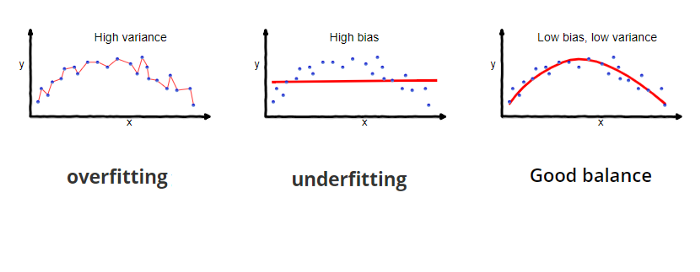
\includegraphics[width=13cm]{bias-variance-tradeoff.png}
\end{figure}


\subsubsection{The Classification Setting}
Many of the previous concepts, including the bias-variance trade-off, transfer over to the classification setting with only some modifications due to the fact that $y_i$ is no longer numerical. Suppose that we seek to estimate $f$ on the basis of training observations $\{(x_1, y_1),...,(x_n, y_n)\}$, where now $y_1,...,y_n$ are qualitative.

The most common approach for quantifying the accuracy of our estimate $\hat f$ is the \textit{training error rate}, the proportion of mistakes that are made if we apply error rate our estimate $\hat f$ to the training observations:

\[
    \frac{1}{n} \sum_{i=1}^n I(y_i  \neq \hat y_i)
\]

Here $\hat y_i$ is the predicted class label for the $i$th observation using $\hat f$. And $I(y_i \neq \hat y_i)$ is an indicator variable that equals 1 if the $i$th observation was misclassified, i.e. $y_i \neq \hat y_i$, and zero it was was classified correctly, i.e.$y_i = \hat y_i$.


The \textit{test error rate} associated with a set of test observations of the form $(x_0, y_0)$ is given by
\[
    Ave(I(y_0 \neq \hat y_0)),
\]
where $\hat y_0$ is the predicted class label. A good classifier minimizes the test error.

\subsubsection{The Bayes Classifier}
To minimize the test error rate, on average, we should simply assign a test observation with predictor vector $x_0$ to the class $j$ for which the conditional probability
\[
    \Pr(Y = j|X = x_0)
\]
is largest. This very simple classifier is called the \textit{Bayes classifier}. In a two-class problem the classification will be class one if $Pr(Y = 1|X = x_0) > 0.5$, and class two otherwise. The line where the probability is exactly 0.5 is called the \textit{Bayes decision boundary}.

The Bayes classifier produces the lowest possible test error rate, called \textit{the Bayes error rate} given by,
\[
1 - E \big( \max_j \Pr(Y = j|X) \big ),
\]
where the expectation averages the probability over all possible values of $X$. The Bayes error rate is analogous to the irreducible error.

In theory we would always like to predict qualitative responses using the Bayes classifier. But for real data, we do not know the conditional distribution of $Y$ given $X$, and so computing the Bayes classifier is impossible. Therefore, the Bayes classifier serves as an unattainable gold standard against which to compare other methods.

\subsubsection{K-Nearest Neighbors}
Given a positive integer $K$ and a test observation $x_0$, the K-nearest neighbors (KNN) classifier first identifies the K points in the training data that are closest to $x_0$, represented by $ \mathcal N_0$. It then estimates the conditional probability for class j as the fraction of points in $ \mathcal N_0$ whose response values equal j:

\[
    \Pr(Y = j|X = x_0) = \frac{1}{K} \sum_{i \in \mathcal N_0} I(y_i = j).
\]

Finally, KNN applies Bayes rule and classifies the test observation $x_0$ to the class with the largest probability.

The choice of $K$ has a drastic effect on the KNN classifier obtained. As $K$ grows, the method becomes less flexible and produces a decision boundary that is close to linear. This corresponds to a low-variance but high-bias classifier. In
general, as we use more flexible classification methods, the training error rate will decline but the test error rate may not.

In both the regression and classification settings, choosing the correct level of flexibility is critical to the success of any statistical learning method. The bias-variance tradeoff, and the resulting U-shape in the test error, can make this a difficult task. 

Nearest Neighbors can be good when the number of variables, $p$, is small, i.e. $p \leq 4$ and for a large number of sample points. It is one of many techniques called smoothers, like kernel and spline smoothing. Unfortunately this method is very poor when $p$ is large, since possible nearby neighbors tend to be far away in high dimensions. This is known as the curse of dimensionality. We need to get a reasonable fraction of the $N$ values of $y_i$ to average in order to bring the variance of our model down. However, as we increase the dimensions, the radius we need to search increases and we lose the efficacy of estimating using local averages

\newpage

\section{Linear Regression}
Linear regression is a very simple approach for supervised learning and is a useful tool for predicting a quantitative response.

\subsection{Simple Linear Regression}

Simple linear regression  is a very straightforward approach for predicting a quantitative response $Y$ on the basis of a single predictor variable $X$. It assumes that there is approximately a linear relationship between $X$ and $Y$. We will sometimes describe this by saying that we are regressing $Y$ on $X$.

\[
    Y \approx \beta_0 + \beta_1 X
\]

$\beta_0$ and $\beta_1$ are two unknown constants that represent the intercept and slope terms in the linear model and are known as its coefficients or parameters.


We may use our training data to produce estimates $\hat \beta_0$ and $\hat \beta_1$ for prediction.

\[
    \hat y  \approx \hat \beta_0 + \hat \beta_1 x
\]

where $\hat y$ indicates a prediction of $Y$ on the basis of $X = x$.


\subsubsection{Estimating the Coefficients}
Let $(x_1, y_1), (x_2, y_2),..., (x_n, y_n)$ represent $n$ observation pairs, each of which consists of a measurement of $X$ and a measurement of $Y$.

We want to find an intercept $\hat \beta_0 $ and a slope $\hat \beta_1$ such that the resulting line is as close as possible to the $n$ data points. The most common definition of closeness involves minimizing the least squares criterion.

Let $\hat y_i = \hat \beta_0 + \hat \beta_1 x_i$ be the prediction for $Y$ based on the $i$th value of $X$. Then $e_i = y_i - \hat y_i$ represents the $i$th residual -- this is the difference between $i$th observed response and its prediction. 

We define the \textit{residual sum of squares (RSS)} as,
\begin{align*}
     RSS &= e_1^2 + e_2^2 + \dots + e_n^2\\
     &=  (y_1 - \hat \beta_0 - \hat \beta_1 x_1)^2 + \cdots + 
     (y_n - \hat \beta_0 - \hat \beta_1 x_n)^2
\end{align*}

The least squares approach chooses $\hat \beta_0 $ and $\hat \beta_1$ to minimize the RSS.

Let $ y \equiv \frac{1}{n} \sum^n_{i=1} y_i$ and $\bar x \equiv \frac{1}{n} \sum_{i=1}^n x_i$ be the sample means. Then the the \textit{least squares coefficient estimates} are given by,

\begin{align*}
    \hat \beta_0 &= \frac{\sum_{i=1}^n (x_i - \bar x) (y_i - \bar y)}{\sum_{i=1}^n (x_i - \bar x)^2} \\ 
    \hat \beta_1 &= \bar y - \hat \beta_1 \bar x
\end{align*}

 
\subsubsection{Assessing the Accuracy of the Coefficient Estimates}

If $f$ is to be approximated by a linear function, then we can write this relationship as a \textit{population regression line},

\begin{align*}
 Y &= f(X) +  \epsilon \\
 Y  &= \beta_0 +  \beta_1 X + \epsilon
\end{align*}
 
Where $\beta_0$ is the intercept, i.e. the expected value of $Y$ when $X = 0$, $\beta_1$ is the slope, i.e.  the average increase in $Y$ in a unit of increase of $X$, and $\epsilon$ is a catch-all error term.
 
The \textit{least squares line} can always be computed using the coefficient estimates, however, the population regression line is unobserved. Fundamentally, the concept of these two lines is a natural extension of the standard statistical approach of using information from a sample to estimate characteristics of an unmeasured large population.
 
The analogy between linear regression and estimation of the mean of a
random variable is an apt one based on the concept of bias. if we could average a huge number of estimates $\hat \mu$ of the true population mean $\mu$ obtained from a huge number of sets of observations, then this average would exactly equal $\mu$. Thus it is an unbiased estimator, i.e. it does not systematically over- or under-estimate the true parameter. 

To determine the accuracy of a sample mean $\hat \mu$ as an estimate of $\mu$, we can find the \textit{standard error}, which roughly tells us the average amount that this estimate differs from the actual value of $\mu$. 

\[
    \text{Var} (\hat \mu) = \text{SE} (\hat \mu ) ^2 = \frac{\sigma^2}{n},
\]

where $\sigma$ is the standard deviation of each of the realizations $y_i$ of $Y$.

To compute the standard errors associated with $\hat \beta_0$ and $\hat \beta_1$,

\begin{align*}
    \text{SE} ( \hat \beta_0 )^2 &= \sigma^2 \big (  \frac{\bar x^2}{(x_i - \bar x)^2}  \big )\\ 
    \text{SE} ( \hat \beta_1 )^2 &= \frac{\sigma^2}{\sum_{i=1}^n (x_i - \bar x)^2} 
\end{align*}

where $\sigma^2 = \text{Var}()$. In general, $\sigma^2$ is not known, but can be estimated from the data. The estimate of $\sigma$ is known as the \textit{residual standard error}, and is given by the formula,
\[
    RSE = \sqrt{RSS/(n - 2)}
\]

Standard errors can be used to compute \textit{confidence intervals}. For example, a  95\% confidence interval is defined as a range of values such that with  95\% probability, the range will contain the true unknown value of the parameter.

For linear regression the confidence interval of the coefficients is given by,
\begin{align*}
    \hat \beta_1 &\pm 2 \cdot \text{SE}(\hat \beta_1)  \\
    \hat \beta_0 &\pm 2 \cdot \text{SE}(\hat \beta_0).
\end{align*}

Standard errors can also be used to perform hypothesis tests on the coefficients. The null hypotheses --  $H_0$ : There is no relationship between $X$ and $Y$, i.e. $\beta_1 = 0$. The alternative hypothesis -- $H_a$ : There is some relationship between $X$ and $Y$, i.e. $\beta_1 \neq 0$. Setting $\beta_1$ removes the $X$ term in  $Y = \beta_0 + \beta_1 X + \epsilon$.  


If $\text{SE}(\hat \beta_1)$ is small, then even relatively small values of $\hat \beta_1$ may provide strong evidence that $\hat \beta_1 \neq 0$  and hence that there is a relationship between $X$ and $Y$. The \textit{t-statistic} given by,
\[
    t = \frac{\hat \beta_1 - 0}{\text{SE}(\hat \beta_1)}
\]
measures the number of standard deviations that $\hat \beta_1$ is away from 0. If there is no relationship between $X$ and $Y$, the t-statistics will have a distribution with n - 2 degrees of freedom. 

The \textit{p-value} corresponds to the probability of observing any number equal to $|t|$ or larger in absolute value, assuming $\beta_1= 0$. A small p-value indicates that it is unlikely to observe such a substantial association between the predictor and the response due to chance, in the absence of any real association, so we can infer that there is an association between the predictor and the response. Then, we can reject the null hypothesis and may declare a relationship between $X$ and $Y$ if the p-value is small enough.

Simply put, a p-value is the probability that random chance generated the data, or (+) another event else that is equal or rarer. The traditional threshold for determining significance of a p-value is $< 0.05$.

\subsubsection{Assessing the Accuracy of the Model}
Given the alternative hypothesis holds, we likely want to quantify the extent to which the model fits the data. A linear regression fit is typically assessed using two related quantities: the residual standard error (RSE) and the $R^2$ statistic.

\subsubsection*{Residual Error}
The RSE is an estimate of the standard deviation of the irreducible error term $\epsilon$. Roughly speaking, it is the average amount that the response
will deviate from the true regression line and is considered a measure of the lack of fit of the model to the data. 

Recall, RSS is the residual sum of squares. Then the RSE is given by,
\[
    RSE = \sqrt{\frac{1}{(n-2)} \text{RSS} } 
    = \sqrt{\frac{1}{(n-2)} \sum_{i=1}^n (y_i - \hat y_i)^2 }.
\]

\subsubsection*{R2 Statistic} 
The $R^2$ statistic provides an alternative measure of fit in terms of the proportion of variance explained and so it always takes on a value between 0 and 1, and is independent of the scale of $Y$ like the RSE. The $R^2$ statistic is a measure of the linear relationship between $X$ and $Y$.

Let $\text{TSS} = (y_i - \hat y)^2$ be the \textit{total sum of squares} and , RSS is the residual sum of squares. Then $R^2$ is given by,
\[
    R^2 =  \frac{\text{TSS} - \text{RSS}}{\text{TSS}} = 1 - \frac{RSS}{TSS}
\]

TSS can be thought of as the amount of variability inherent in the response before the regression is performed while RSS measures the amount of variability that is left unexplained after performing the regression. TSS - RSS measures the amount of variability in the response that is explained (or
removed) by performing the regression, and $R^2$ measures the proportion of variability in $Y$ that can be explained using $X$.

An $R^2$ statistic that is close to 1 indicates that a large proportion of the variability in the response has been explained by the regression, while the converse holds for a value close to 0. The $R^2$ statistic is similar to correlation, but holds for a between a larger number of variables.

\subsection{Multiple Linear Regression}
We can handle multiple predictors by giving each predictor a separate slope coefficient in a single model. In general, suppose that we have $p$ distinct predictors. Then the multiple linear regression model takes the form,

\[
    Y = \beta_0 + \beta_1 X_1 + \beta_2 X_2 + \dots + \beta_p X_p + \epsilon,
\]
where $X_j$ represents the $j$th predictor and $\beta_j$ quantifies the association between that variable and the response, namely the average effect on $Y$ of a one unit increase in $X_j$ , holding all other predictors fixed.

\subsubsection{Estimating the Regression Coefficients}

Given estimates $\hat \beta_0, \hat \beta_1,..., \hat \beta_p$, we can make predictions using the formula,
\[
     \hat y= \hat \beta_0, \hat \beta_1 x_1,..., \hat \beta_p x_p.
\]
We choose $\beta_0, \beta_1,...,\beta_p$ to minimize the sum of squared residuals,
\begin{align*}
    RSS &= \sum_{i=1}^{n} (y_i - \hat y_i)^2 \\
    &=  \sum_{i=1}^{n}(y_i - \hat \beta_0 - \hat \beta_1 x_1,..., \hat \beta_p x_p)^2.
\end{align*}
The values $\hat \beta_0, \hat \beta_1 x_1,..., \hat \beta_p x_p$ that minimize the above equation are the multiple least squares regression coefficient estimates. These values are most easily represented using matrix algebra and will be revisited later.

\subsubsection{Some Important Questions}
\begin{enumerate}
    \item Is at least one of the predictors $X_1, X_2,...,X_p$ useful in predicting the response?
    \item Do all the predictors help to explain $Y$, or is only a subset of the predictors useful?
    \item How well does the model fit the data? 
    \item Given a set of predictor values, what response value should we predict, and how accurate is our prediction?
\end{enumerate}

\subsubsection*{Is There a Relationship Between the Response and Predictors?}
In the multiple regression setting with $p$ predictors, we need to ask whether all of the regression coefficients are zero. The null hypothesis becomes,
\[
    H_0 : \beta_1 = \beta_2 = \dots = \beta_p = 0.
\]

This hypothesis test is performed by computing the \textit{F-statistic}.
\[
    F = \frac{(\text{TSS} - \text{RSS})/p }{\text{RSS}/ (n-p-1)}
\]

When there is no relationship between the response and predictors, one would expect the F-statistic to take on a value close to 1. On the other hand, if $H_a$ is true (i.e. at least one $\beta_j$ is non-zero.), then $E{(\text{TSS} - \text{RSS})/p} > \sigma^2$, so we expect $F$ to be greater than $1$.

The approach of using an F-statistic to test for any association between the predictors and the response works when $p$ is relatively small, and certainly small compared to $n$. However, sometimes we have a very large number of variables. If $p>n$ then there are more coefficients $\beta_j$ to estimate than observations from which to estimate them. In this case we cannot even fit the multiple linear regression model using least squares, so the F-statistic cannot be used. Approaches like forward selection, discussed later, can be used instead.

\subsubsection{Deciding on Important Variables}
The first step in a multiple regression analysis is to compute the F-statistic and to examine the associated p-value. If we conclude on the basis of the p-value that at least one of the predictors is related to the response, then it is natural to wonder which are the relevant ones. The task of determining which predictors are associated with the response, in order to fit a single model involving only those predictors, is referred to as \textit{variable selection}, discussed more in detail in chapter 6.

There are a total of $2^p$ models that contain subsets of $p$ variables. . In general, we cannot consider all $2^p$ models, and instead we need an automated and efficient approach to choose a smaller set of models to consider. There
are three classical approaches for this task:
\begin{enumerate}
    \item \textit{Forward selection} -- We begin with the null model, i.e. a model that contains an intercept but no predictors. We then fit p simple linear regressions and add to the null model the variable that results in the lowest RSS. We then add to that model the variable that results in the lowest RSS for the new two-variable model. This approach is continued until some stopping rule is satisfied.
    
    \item \textit{Backward selection} -- We start with all variables in the model, and remove the variable with the largest p-value—that is, the variable  that is the least statistically significant. The new ($p - 1$)-variable model is fit, and the variable with the largest p-value is removed. This procedure continues until a stopping rule is reached, i.e. when  all remaining variables have a p-value below some threshold.
    
    \item Mixed selection -- This is a combination of forward and backward selection. We start with no variables in the model, and as with forward selection, we add the variable that provides the best fit. Since the p-values for variables can become larger as new predictors are added to the model, if at any point the p-value for one of the variables in the model rises above a certain threshold, then we remove that variable from the model. We continue to perform these forward and backward steps until all variables in the model have a sufficiently low p-value.
\end{enumerate}

Backward selection cannot be used if $p>n$, while forward selection can
always be used. Forward selection is a greedy approach, and might include
variables early that later become redundant. Mixed selection can remedy
this.

\subsubsection*{Model Fit}
In multiple linear regression, $R^2 =  Cor(Y, \hat Y)^2$,  the square of the correlation between the response and the fitted linear model. $R^2$ will always increase when more variables are added to the model, even if they are only weakly associated with the response.  This is due to the fact that adding another variable to the least squares equations must allow us to fit the training data more accurately, so the R2 statistic, which is also computed on the training data, must increase.

\subsubsection*{Predictions}
After fitting a regression model, there are three sorts of uncertainty associated with a prediction.
\begin{enumerate}
    \item There will be some inaccuracy in the coefficient estimates related to the reducible error of using the least squares plane. We can compute a confidence interval in order to determine how close $\hat Y$ will be to $f(X)$.
    \item There is potentially an additional source of reducible error, called \textit{model bias}, from using a linear model to represent complex non-linear data.
    \item The will be some amount of irreducible or random error in the model.  \textit{Prediction intervals} are used to incorporate both the error in the estimate for $f(X)$ (the reducible error) and the uncertainty as to how much an individual point will differ from the population regression plane (the irreducible error). 
\end{enumerate}


\subsection{Other Considerations in the Regression Model}
\subsubsection{Qualitative Predictors}
\subsubsection*{Predictors with Only Two Levels}
If a qualitative predictor (also known as a factor) only has two levels, or possible values, then incorporating it into a regression model is very simple. We simply create an indicator or dummy variable that takes on two possible numerical values, i.e. (0 or 1) and use this variable as a predictor in the regression equation.

\subsubsection*{Qualitative Predictors with More than Two Levels}
In this situation, we can create additional dummy variables. There will always be one fewer dummy variable than the number of levels. The level with no dummy variable is known as the \textit{baseline}.

\subsubsection{Extensions of the Linear Model}
Two of the most impactful assumptions in the standard linear regression model state that the relationship between the predictors and response are additive and linear. The \textit{additive} assumption means that the effect of changes in a predictor $X_j$ on the response Y is independent of the values of the other predictors. The \textit{linear} assumption states that the change in the response $Y$ due to a one-unit change in $X_j$ is constant, regardless of the value of $X_j$.

\subsubsection*{Removing the Additive Assumption}
One way of extending this model to allow for interaction effects is to include a third predictor, called an interaction term, which is constructed by computing the product of X1 and X2.
\begin{align*}
    Y &= \beta_0 + \beta_1 X_ 1 + \beta_2 X_2 + \beta_3 X_1 X_2 + \epsilon \\
    &= \beta_0 + (\beta_1 + \beta_3 X_2)X_1 + \beta_2 X_2 + \epsilon \\
    &= \beta_0 + \Tilde \beta_1 X_1 + \beta_2 X_2 + \epsilon
\end{align*}
Then, adjusting $X_2$ will change the impact of $X_1$ on $Y$.

The \textit{hierarchical principle} states that if we include an interaction in a model, we should also include the main effects, even if the p-values associated with their coefficients are not significant.
 
\subsubsection*{Non-linear Relationships}
In some cases, the true relationship between the response and the predictors may be nonlinear. A simple way to directly extend the linear model to accommodate non-linear relationships is to use \textit{polynomial regression}, in which we include polynomial functions of the predictors in the regression model.

\subsubsection{Potential Problems}
\begin{enumerate}
    \item Non-linearity of the response-predictor relationships.
    
        Residual plots are useful graphical tool for identifying non-linearity. If there is a strong pattern in the  plot of the residuals, $e_i = y_i - \hat y_i$, versus the predictor $x_i$, there may be a problem with some aspect of the linear mode.
    
    \item Correlation of error terms.
    
         In general, the assumption of uncorrelated errors is extremely important for linear regression as well as for other statistical methods.
        
        If there is correlation among the error terms, then the estimated standard errors will tend to underestimate the true standard errors, confidence and prediction intervals will be narrower than they should be, and p-values associated with the model will be lower than they should be.  Such correlations frequently occur in the context of time series data.
        
        We can plot the residuals from our model as a function of time and if the errors are uncorrelated, then there should be no discernible pattern. Otherwise we may find that \textit{tracking} exists, i.e. adjacent residuals often have similar values.
    
    \item Non-constant variance of error terms.
        
        An important assumption is that error terms have constant variance, i.e. $ \text{Var}(i) = \sigma^2$.  One can identify non-constant variance, a.k.a. heteroscedasticity, from the presence of a funnel shape in the residual plot.
        
        A simple remedy may be to fit our model by \textit{weighted least squares}, with weights proportional to the inverse weighted variances.
    
    \item Outliers.
    
    A point for which $y_i$ is far from the value predicted by the model can occur for many reasons, possibly as a result  of incorrect recording of an observation.
    It is typical for an outlier that does not have an unusual predictor value to have little effect on the least squares fit, but may have an effect on the RSE, used to compute all confidence intervals or p-values, as well as $R^2$. 
    
    Residual plots can be used to identify outliers, but in practice, it can be difficult to decide how large a residual needs to be before we consider the point to be an outlier. Instead, we can plot the \textit{studentized residuals}, computed by dividing each residual $e_i$ by its estimated standard error. Observations whose studentized residuals are greater than 3 in absolute value are possible outliers and can be removed or examined to determine a deficiency with the model, such as a missing predictor.
    
    \item High-leverage points.
    
    In contrast to outliers, observations with \textit{high leverage} have an unusual value for $x_i$. Removing a high leverage observation has a much more substantial impact on the least squares line than removing the outlier.
    
    To quantify an observation’s leverage, we compute the \textit{leverage statistic}. The leverage statistic $h_i$ is always between $1/n$ and $1$, and the average leverage for all the observations is always equal to $(p + 1)/n$. For a simple linear regression,
    \[
        h_i =  \frac{1}{n} \frac{(x_i - \bar x)^2}{\sum_{i' = 1}^n (x_i - \bar x)^2}
    \]
    
    \item Collinearity.
    
    \textit{Collinearity} refers to the situation in which two or more predictor variables are closely related to one another. In the regression context, it can be difficult to separate out the individual effects of collinear variables on the response and reduces the accuracy of the estimates of the regression coefficients. This causes the standard error for $\hat \beta_j$ to grow and the t-statistic to decline which in turn means the power of the hypothesis test - the probability of correctly detecting a non-zero coefficient - is reduced by collinearity.
    
    A simple way to detect collinearity is to look at the correlation matrix of the predictors, though this may not always work. In particular, it is possible for collinearity to exist between three or more variables in what's called \textit{multicollinearity}. In this situation it's better to compute the \textit{variance inflation factor} (VIF), the ratio of the variance of $\hat \beta_j$ when fitting the full model divided by the variance of $\hat \beta_j$ if fit on its own. A VIF value of 1indicates the complete absence of collinearity, a VIF value that exceeds 5 or 10 indicates a problematic amount of collinearity.
    
    \[
        VIF(\hat \beta_j ) = \frac{1}{1-R^2_{X_j|X_{-j}}}
    \]
    where $R^2_{X_j|X_{-j}}$ is the $R^2$ from a regression of $X_j$ onto all of the other predictors.
    
    To mitigate collinerarity, we may drop one of the problematic variables from the regression, which will also reduce redundancy. Alternatively, we may combine the collinear variables together into a single predictor.
    
\subsection{Comparison of Linear Regression with K-Nearest Neighbors}
Linear regression is an example of a parametric approach and has many advantages: they are often easy to fit, the coefficients have simple interpretations, and tests of statistical significance can be easily performed. But parametric methods do have a disadvantage: by construction, they make strong assumptions about the form of $f(X)$. 

In contrast, non-parametric methods do not explicitly assume a parametric form for $f(X)$, and thereby provide an alternative and more flexible approach for performing regression. 

One of the simplest and best-known non-parametric methods is \textit{K-nearest neighbors regression} (KNN regression), which is closely related to the KNN classifier.

Given a value for $K$ and a prediction point $x_0$, KNN regression first identifies the $K$ training observations that are closest to $x_0$, represented by $\mathcal N_0$. It then estimates $f(x_0)$ using the average of all the training responses in $mathcal N_0$. In general, the optimal value for K will depend on the bias-variance tradeoff.

\[
    \hat f (x_0) = \frac{1}{K} \sum_{x_i \in \mathcal N_0} y_i.
\]

The parametric approach will outperform the nonparametric approach if the parametric form that has been selected is close to the true form of $f$. Even when the true relationship is highly non-linear, KNN may still provide inferior results to linear regression. A decrease in performance as the dimension increases is a common problem for KNN, and results from the fact that in higher dimensions there is effectively a reduction in sample size. As a general rule, parametric methods will tend to outperform non-parametric approaches when there is a small number of observations per predictor.

\section{Classification}

\section{Resampling Methods}

\section{Linear Model Selection and Regularization}

\section{Moving Beyond Linearity}

\section{Tree-based Methods}

\section{Support Vector Machines}

\section{Unsupervised Learning}

\end{enumerate}


\comment{
- left off: pg 47, video:  Lect3 4b 110613
- 
}


\begin{thebibliography}{}
\bibitem[]{}
Gareth James, Daniela Witten, Trevor Hastie, Robert Tibshirani. An Introduction to Statistical Learning : with Applications in R. New York :Springer, 2013.


http://faculty.marshall.usc.edu/gareth-james/ISL/ISLR\%20Seventh\%20Printing.pdf

% https://www.dataschool.io/15-hours-of-expert-machine-learning-videos/


\bibitem[]{}
https://arxiv.org/pdf/1010.3162.pdf

\bibitem[]{}
http://bactra.org/notebooks/learning-theory.html

\end{thebibliography}


\end{document}
